% !TeX spellcheck = en_EN-English

One of sub-task for prediction of patient future costs is to embed each patient record into numerical vector that would be understandable for neural network. Some of patient information like age are easy to embed as they are ordered numerical values to begin with, while others are much more tricky. More specifically we needed to figure our how to embed three main information: diagnosis, medical procedure and prescribed drug.

\section{Diagnosis embedding}

Base diagnose information we embed was ICD-10-CM code of disease.ICD-10-CM stands for "International Classification of Diseases, Tenth Revision, Clinical Modification" and is used to code and classify medical diagnoses \cite{cdcICD10CM} most precisely version of this code that is used in Slovakia and is better known by the acronym MKCH-10-SK (Medzinárodná klasifikácia chorôb) \cite{ncziMKCH}.\\

\begin{figure}[!h]
	\centering
	
	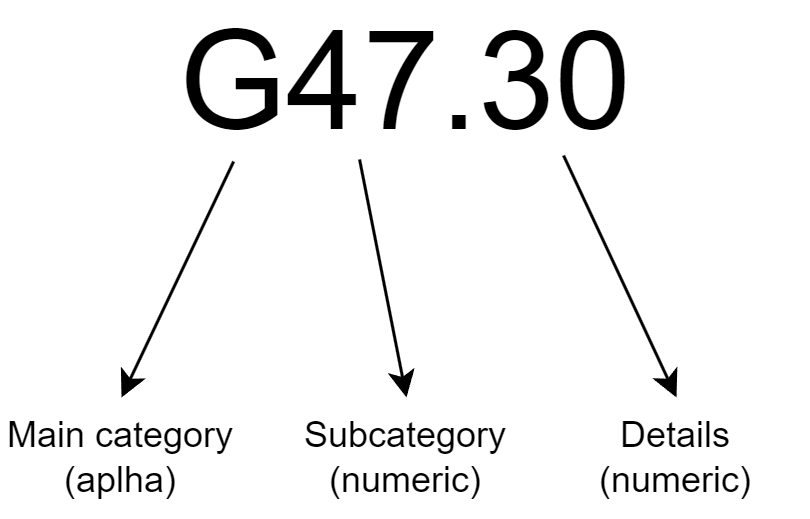
\includegraphics[width=0.8\textwidth]{images/ICD-10-CM.png}
	
	\caption{Structure of MKCH-10 code}
	\label{fig:icd-10-cm}
\end{figure}

This code consist of three parts as shown on image \ref{fig:icd-10-cm}. First part is one letter that encodes main categories of diseases also known as chapter, for example codes starting with G are diseases of the nervous system. 
After that there is two numeric characters that further specify subcategory of disease such as codes from G40 to G47 which are episodic and paroxysmal disorders and specifically G47 are sleep disorders. 
We can see that episodic and paroxysmal disorders are only up to G47, meaning that theoretically there can exist subgroups G48 and G49 which have 4 in second position but does not belong to same G4 subcategory as G40 or G47 \label{mkch_subdiv}. Thankfully this is not the case and in cases like this when higher lower subcategory (like G4) does not have 10 lower level subcategories (like G47) these subcategories does not exist at all and in case it have more than 10 lower level subcategories it gets multiple consecutive high level subcategories, for example disorders of other endocrine glands spans from E20 to E35. 
Then code contains dot after which there are characters that further describe details of disease such as etiology, anatomic site and severity. Official documentation of ICD-10-CM codes stands that codes can be up to 7 characters long meaning that after first three characters specifying category there can be up to 4 alphanumeric to further specify the disease \b{CITE}, however Slovak version MKCH-10 codes contains at most two numeric characters to specify disease \b{cite} and these details are organized in a way where the first position conveys higher-level information than the second, for example G47.3 is sleep apnea and G47.30 is primary central sleep apnea.
\\

To embed this code we firstly split it into it's three parts and embed each part separately. After that we concatenated embedding of each part to get final embedding of disease.
To embed main category we generated vector containing random numbers from range [-0.5, 0.5] using uniform distribution for each letter of English alphabet (all main categories). We used random vectors in order to have relatively similar distance between any two main categories since there are no particular relationships between these categories, we were thinking also about using one-hot encoding which would make distance between each two categories perfectly same but we didn't do it since it would have restricted length of vector. 
In embedding second part which is subcategory we used different approach, where to each number between 00 and 99 (all possible values of this part) we assign linearly number between -0.5 and 0.5, meaning subcategory 00 would get -0.5 category 50 would get 0 and category 99 would get 0.5, we choose these boundaries in order to match mean and variance of of numbers generated for main category. This assigned number was then repeated multiple times to create vector. This approach has advantages and disadvantages. Advantage is that we can be sure that closely related disease subgroups like G46 and G47 would get close embedding since their subgroup codes are close on number line. However there are also two disadvantages, first is that G49 and G50 would be similarly close as G46 and G47, but thankfully in a most cases either X9 code doesn't exist at all, creating a gap, or if X9 code exist it belong to category that go past X on as higher level subgroup. Another disadvantage is that distance between two higher level subgroups can vary quite dramatically even though in reality there might not be reason for that difference in distance. For example, using this approach higher level subgroup G40-G47 is much closer to subgroup G50-G59 than to G80-G83.
Finally to embed details we decided to use same approach as for subgroups since these codes work similarly, only difference was that not all codes had second level details, in such cases we add 5 as a proxy in order to minimize average distance from all potential codes with same first level details code that contain second level detail information while also maximizing average distance to different first level detail codes.
Final after embedding each part final embedding is created as their concatenation, to encode importance of each part in final embedding we gave them different lengths, this works thanks to the fact that each value in each of vector have same mean and same variance. Main category, the most important part, got vector of length 26, subcategory part got length 8 and finally details got length 2.
Showcase of resulting embedding can be seen on image \ref{fig:diag_emb_show} where each part is highlighted by different color and all values are rounded to two decimal.
In order to confirm that our embedding has desired properties we computed similarity of embedding of multiple codes. As similarity function we choose simple multiplicative inverse of Euclidean distance. In table \ref{tab:diag_emb_show} we can see results. Highest similarity was between codes G47.30 and G40.09 which is expected since they belong to same main category and very close subcategory, second highest was between H40.09 and H18.80 which are only other combination that belong to same main category, this confirms that main category has biggest impact since this similarity is significantly higher than that between G40.09 and H40.09 which differ only main category.

\begin{figure}[!h]
	\centering
	
	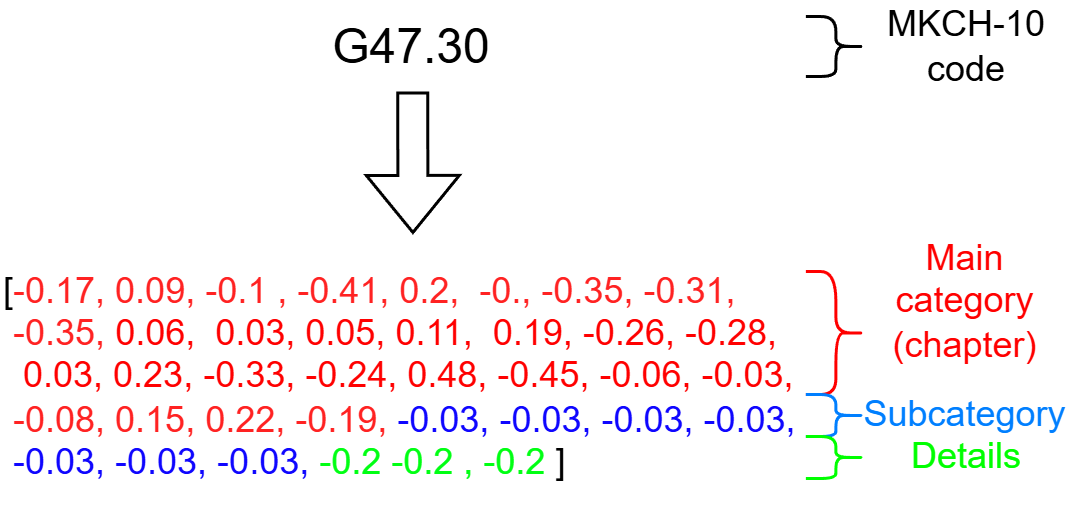
\includegraphics[width=0.8\textwidth]{images/diagnosis_embed_showcase.png}
	
	\caption{Showcase of resulting embedding of specific diagnosis (rounded to two decimal places)}
	\label{fig:diag_emb_show}
\end{figure} 


\begin{table}[!h]
	\centering
	\begin{tabular}{|l|l|l|}
		\hline
		Code A & Code B & Similarity \\ \hline
		G47.30 & G40.09 & 2.77       \\ \hline
		G47.30 & H40.09 & 0.53       \\ \hline
		G47.30 & H18.80 & 0.46       \\ \hline
		G40.09 & H40.09 & 0.54       \\ \hline
		G40.09 & H18.80 & 0.45       \\ \hline
		H40.09 & H18.80 & 0.84       \\ \hline
	\end{tabular}
	\caption{Table of similarities of multiple chosen MKCH-10 codes}
	\label{tab:diag_emb_show}
\end{table}  

\section{Drug embedding}

Similarly to diagnosis, to embed drug information we embed international code associated to these drug. In case of drugs it was Anatomical Therapeutic Chemical classification system also known under abbreviation ATC. In a same way as MKCH-10 code this code can be split into multiple parts where each next part contains finer information. It contains of 5 parts or levels. First level encodes main anatomical or pharmacological groups. There are fourteen such groups, encoded by single letter, which are shown in the figure \ref{fig:atc_l1}. Then second level encodes pharmacological or therapeutic subgroup using two digit number, after that there two levels that further specify pharmacological, therapeutic or even chemical subgroup, these two levels are both encoded using single letter each. Final fifth encoded with two digit number contains information about specific chemical substance inside drug.

\begin{figure}[!h]
	\centering
	
	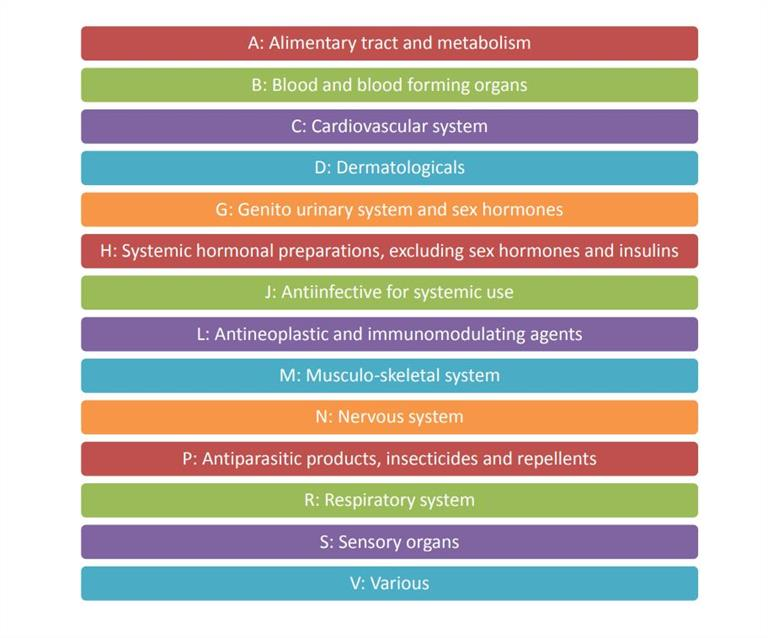
\includegraphics[width=0.8\textwidth]{images/atc_l1_classification_who.jpg}
	
	\caption{Fourteen main anatomical or pharmacological groups and their corresponding first level ATC code \cite{atc_who}}
	\label{fig:atc_l1}
\end{figure}



Embedding was done in very similar way as in diagnosis embedding with one difference and that is that each level is embed using random vectors because none of the levels contains sub-grouping that would require to numerically or alphabetically closer codes to have closer embedding (see \ref{mkch_subdiv} subgroup codes).


